\section{Metod}

 

Valet av metod grundar sig i tidigare uppställningar för liknande laborationer, samt en laborations uppställning som visas av handledaren Duygu Yilmaz\cite{Aarabi-Karasgani2010}. Experimentuppställningen består av en trehalsad rundbottenskolonn som befinner sig i ett vattenbad på en värmeplatta med magnetomrörning. Till de tre halsarna så är en av halsarna försedd med en kork, en med en termometer, och slutligen en med kondensor se i Figur \ref{fig:labupp}, samt Figur \ref{fig:labbild}. Temperaturen, ration mellan vätska och fast ämne, samt koncentration på syran väljs beroende på vilken kedja av experiment som utförs, se tabell \ref{tab:metodtab}. Lakningen sker genom att 1 gram av LD-slagget tillsätts till H$_{2}$SO$_{4}$, som är förvärmt till rätt temperatur för det experimentet. Omrörningen har bestämts till 360 rpm. Provet lakas i 2 timmar och provtagningen sker i intervallerna 30 minuter, 60 minuter, 120 minuter. Vid provtagning plockas 1 ml upp av provet. Efter att lakningen är gjord så filteras provet med en Büchner tratt med ett glasfilter och ett pappersfilter. Provet är nu efter detta redo för att analyseras med en AAS. 
\begin{figure}[H]
    \centering
    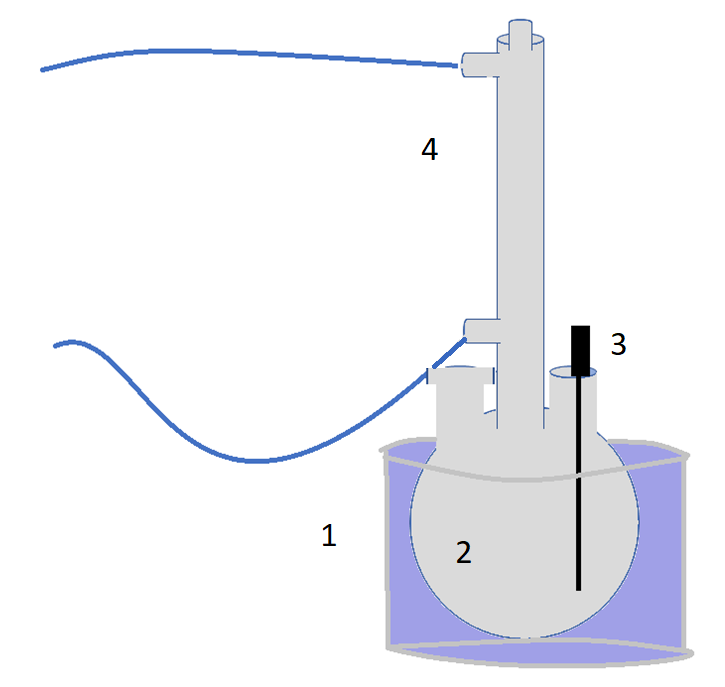
\includegraphics[scale=0.4]{labbupp.png}
    \caption{Laborations uppställningen i nuläget. 1. Vattenbad som värms upp med en värmeplatta. 2. Trehalsad rundbottenskolonn. 3. Termometer som är kopplad till värmeplatten. 4. Kondensor.    }
    \label{fig:labupp}
\end{figure}

\begin{table}[H]
\caption{Premilinär test uppställning.}
\begin{tabular}{|l|c|c|c|}
\hline
\textbf{\begin{tabular}[c]{@{}l@{}}Parametrar\end{tabular}}              & \multicolumn{1}{l|}{\textbf{\begin{tabular}[c]{@{}l@{}}H$_{2}$SO$_{4}$ \\ koncentration [M]\end{tabular}}} & \multicolumn{1}{l|}{\textbf{\begin{tabular}[c]{@{}l@{}}Ratio mellan vätska \\ fast och  [ml/g]\end{tabular}}} & \multicolumn{1}{l|}{\textbf{\begin{tabular}[c]{@{}l@{}}Laknings\\ Temperatur  [$\degree$C]\end{tabular}}} \\ \hline
\textbf{\begin{tabular}[c]{@{}l@{}}H$_{2}$SO$_{4}$ \\ koncentration [M]\end{tabular}}    & 3,4,5                                                                                                    & 25:1                                                                                                           & 70                                                                                                        \\ \hline
\textbf{\begin{tabular}[c]{@{}l@{}}Ratio mellan vätska\\ och fast [ml/g]\end{tabular}} & 3                                                                                                          & 25:1, 50:1, 100:1                                                                                            & 70                                                                                                        \\ \hline
\textbf{\begin{tabular}[c]{@{}l@{}}Laknings \\ Temperatur  [$\degree$C]\end{tabular}}    & 3                                                                                                          & 25:1                                                                                                           & 50, 60, 70, 80                                                                                               \\ \hline
\end{tabular}
\label{tab:metodtab}
\end{table}

 Ett flertal metoder kommer att användas för att analysera proverna. Atomabsorptionsspektroskopi, AAS, och röntgenkristallografi, XRD från engelska X-ray diffraction, och svepelektronmikroskopi, SEM. De olika metoderna används för olika delar av arbetet. AAS används för att undersöka om vanadin har lakats ur LD-slagget. XRD kommer att användas för att analysera kristallstrukturen av LD-slagget före och efter att det har rostats och vid olika intervaller under rostningen för att se sammansättningen av de olika ämnena i kristallen. Slutligen så kommer SEM användas för att se var i LD-slagget som de olika ämnena befinner sig i slaggpartiklarna. 

En litteraturstudie ska ske parallellt med laborationerna för att kunna ge möjlighet till djupare inlärning och förklaring av ämnet. Detta innebär användningsområden av vanadin, användadet av LD-slagg och dess deponering i nuläget. Även vilka fördelar och nackdelar processen har och vad det kan göra för samhällsnytta inför i framtiden. 